\documentclass[11pt, onecolumn, oneside, reqno]{article}
\usepackage[english]{babel}
\usepackage{geometry}                		% See geometry.pdf to learn the layout options. There are lots.
\geometry{a4paper}
%\geometry{landscape}                		% Activate for rotated page geometry
\usepackage[parfill]{parskip}
\usepackage{graphicx} % Use pdf, png, jpg, or eps§ with pdflatex; use eps in DVI mode, TeX will automatically convert eps --> pdf in pdflatex		
\usepackage{amsmath, mathtools}  
%\usepackage{bbm}              %$\mathbbm{Q}$
%\usepackage{mathrsfs}         %$\mathscr{L}$
%\usepackage{apacite}
\usepackage[font=small]{caption}
%\captionsetup[table]{skip=2pt}
\usepackage{abstract}
% hyperref should be the last package declaration
\usepackage[colorlinks=true, urlcolor=blue, linkcolor=blue]{hyperref}

\title{Deep Learning Project: Follow Me! \\ Robotics Nanodegree, Udacity}

\author{Stephan Hohne}
\date{November 9, 2017}

\begin{document}
\maketitle

\begin{abstract}
This report describes my solution of the deep learning project. First I describe the convolutional network as applied to the given semantic segmentation task. Then I describe the data collection process, the network architecture and training process. In the last section I present the results and discuss the performance of the tested models. The code for this project can be found in \href{https://github.com/S2H-Mobile/RoboND-DeepLearning-Project-Solution}{this repository}.
\end{abstract}

\tableofcontents

\newpage

\listoftables

\listoffigures

\newpage

\section{Fully Convolutional Network for Semantic Segmentation}
\label{sec:fcn_description}
For writing this section I used what I learned in the classroom and references \cite{CS231n, Xception, MobileNets}.

\subsection{Overview}
The goal of this project is to build and train a neural network that enables a drone to follow a person in a simulated environment.

The network is supposed to do semantic segmentation of the given image and detect the location of the hero person in the scene. To accomplish this goal, each pixel is classified as either belonging to the target person or being part of another person or not being part of any person. If the model were to distinguish more target types (dog, cat, car, etc.), the number of output classes would change. The depth of the final layer would have to be adjusted accordingly, and the network trained with additional labeled image data containing these target types.

The image segmentation task can be accomplished with a fully convolutional network (FCN). Such architectures consist of convolution layers exclusively.

\subsubsection*{Encoding and Decoding}
The architecture used in this project is comprised of an encoding and a decoding stage. The encoder gradually reduces the spatial size of the image with pooling layers. The decoder scales the feature maps back up to the original size.

The convolution layers in the encoder extract feature maps from the image data. So they learn details about the image which will be used for segmentation. The complexity of the encoded features increases with the number of layers.

The pooling layers in the encoder perform a downsampling operation along the width and height of the image. This enables the model to generalize to unseen input, and it reduces the risk of overfitting to the training data. The drawback of pooling is that the original image gets coarse-grained. The resolution is lowered and some of the corresponding spatial information is lost.

The purpose of the decoder block is to scale the low resolution feature maps up to the original image resolution, so that the network can classify all of the pixels in the input image. 
 
The upsampling operation fills the gaps between missing pixel values by interpolation. The information which was lost during pooling can't be fully restored by the upsampling operation, and the decoder can't recover the spatial resolution completely.
 
To help the decoder recover the object details, skip connections are introduced. They connect the high resolution encoder layers directly to the decoder, so that some of the information from those layers can be restored.  

\subsubsection*{Depthwise Separable Convolution}
For writing this section I read section 3 in \cite{MobileNets} and section 1 in \cite{Xception}.

The encoder architecture is built as a depthwise separable convolution. The standard convolution layer is factorized into a depthwise convolution looking at spatial correlations and a $1 \times 1$ pointwise  convolution that detects correlations in the color channels. The underlying assumption is that the information encoded in the spatial dimensions is independent of the information in the depth channel.

So the last layer in the encoder is a regular convolution with kernel size $1 \times 1$ and stride of $1$. So each neuron has a receptive field of only one pixel, therefore the input and output volumes have equal height and width. The output tensor is of size $H \times W \times M$ with the height and width and depth of the input volume. In comparison, a fully connected final layer would reduce the output into a single vector, where the class scores are arranged along the depth dimension. So the output tensor of the final layer would have size $1 \times 1 \times D$ where $D$ is the number of classes.

This depthwise factorization has the advantage of drastically reducing the model size and the computational cost. The efficiency of the encoder network improves, and the number of parameters is reduced. The drawback is that the assumption that the color channel information is decoupled from the spatial information might not hold for the actual image data we are using in our model.

\subsection{Implementation}
The encoding stage consists of two separable convolutions followed by a regular $1 \times 1$ convolution with a stride of one and same padding.

The purpose of the decoder block is to scale the encoder output up to the size of the input image and decode the data stored in the previous layers. It is comprised of three parts.
\begin{itemize}
\item A non-trainable bilinear upsampling layer. The value of an output pixel is determined by interpolation of its nearest neighbors in the input.
\item A non-trainable concatenation layer. It implements skip connections and thereby retains some of the information from the previous higher resolution layers.
\item One or more separable convolutions which learn from the data stored in the concatenated layer.
\end{itemize}

The final layer of the model is a regular convolution with softmax activation. It assigns class probabilities to each pixel in the image.

\section{Data Collection}
\label{sec:data_collection}
\begin{figure}
\noindent
\makebox[\textwidth]{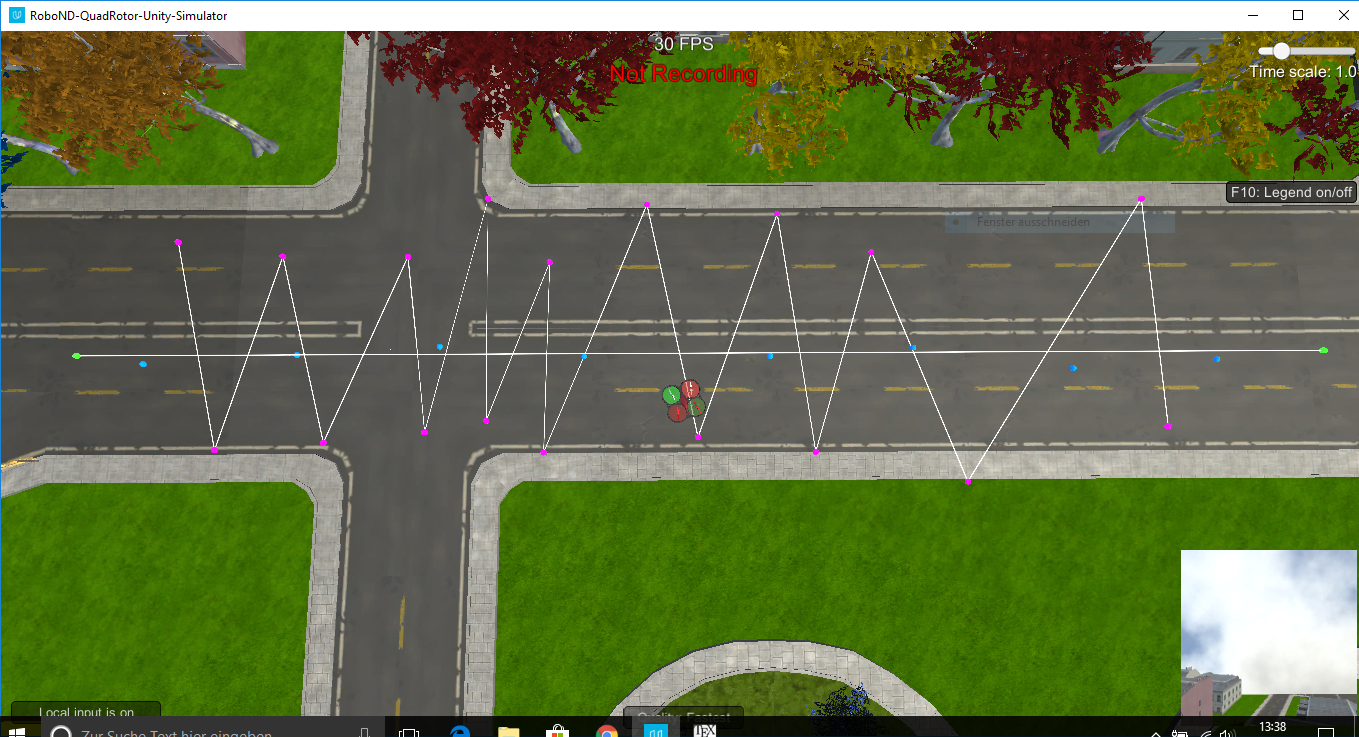
\includegraphics[width=\textwidth]{images/data_collection_target_run_1.png}}
\caption[Paths for data collection run $1$]{Drone and hero paths for data collection run $1$.}
\label{img:data_collection_run_1}
\end{figure}

\begin{figure}
\noindent
\makebox[\textwidth]{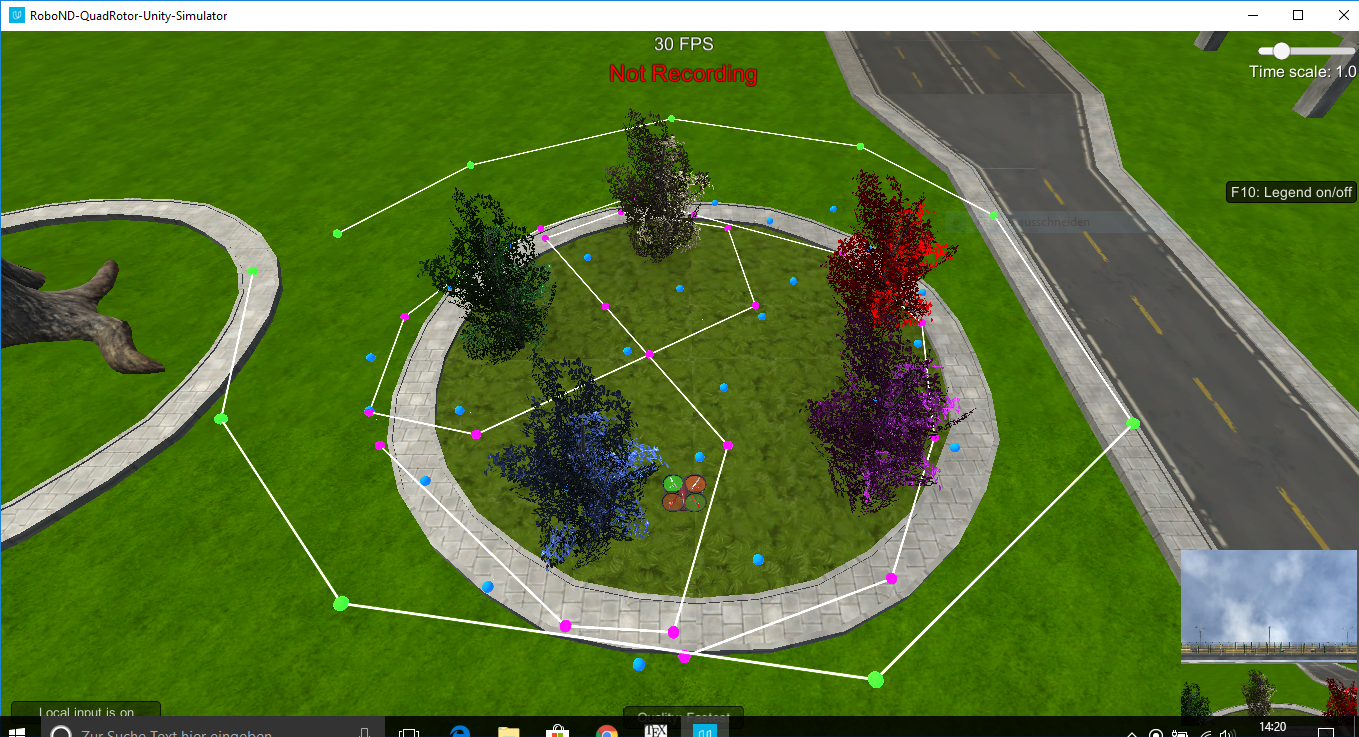
\includegraphics[width=\textwidth]{images/data_collection_target_run_2.png}}
\caption[Paths for data collection run $2$]{Drone and hero paths for data collection run $2$.}
\label{img:data_collection_run_2}
\end{figure}
I collected image data in the \texttt{QuadRotor} simulator. The goal was to collect sequences that the drone will encounter in application, with the target person in it. I ran two different path layouts.
\begin{enumerate}
\item Drone patrols directly over the hero. The paths are laid out such that the drone follows a straight line and the hero zigzags around that line, as shown in figure \ref{img:data_collection_run_1}.
\item The drone circles around the hero and many distracting people. See figure \ref{img:data_collection_run_2}.
\end{enumerate}

I collected $270$ data sets in the first run and $186$ data sets in the second run. One such data set consists of four camera images. I ran the image processing script \href{https://github.com/S2H-Mobile/RoboND-DeepLearning-Project-Solution/blob/master/code/preprocess_ims.py}{\texttt{preprocess\_ims.py}} which returned $456$ image/mask combinations. I used these data points as additional training data, so I added them to the training data set and left the data sets for validation and evaluation as they were.

The resulting new training data set \texttt{train\_combined.zip} (file size $56.7$\,MB) consists of $4587$ image/mask combinations and can be downloaded from the \href{https://github.com/S2H-Mobile/RoboND-DeepLearning-Project-Solution/tree/master/data}{repository}. I used this data set to train the network as described in section \ref{sec:training_additional_data}. The results of this experiment can be found in table \ref{tbl:collected_data_experiment}.

\section{Network Architecture and Training}
I trained the network on a AWS \texttt{p2.xlarge} instance with the ​Udacity​ ​Robotics​ ​Laboratory​ ​Community​ ​AMI installed. The training code can be found in the notebook \href{https://github.com/S2H-Mobile/RoboND-DeepLearning-Project-Solution/blob/master/code/model_training.ipynb}{\texttt{model\_training.ipynb}}.

The evaluation is done using the intersection over union metric as the final score.

I conducted three different experiments in order to find the combination of network architecture and hyperparameter values that achieves the highest possible final score. I used the data sets \href{https://s3-us-west-1.amazonaws.com/udacity-robotics/Deep+Learning+Data/Lab/train.zip}{\texttt{train.zip}}, \href{https://s3-us-west-1.amazonaws.com/udacity-robotics/Deep+Learning+Data/Lab/validation.zip}{\texttt{validation.zip}} and \href{https://s3-us-west-1.amazonaws.com/udacity-robotics/Deep+Learning+Data/Project/sample_evaluation_data.zip}{\texttt{sample\_evaluation\_data.zip}} as a reference, so the results of the training runs are comparable.

For all training runs described here, the number of validation steps is $50$ and the number of workers is $4$. 

\subsection{Architecture Parameters}
\label{sec:reference_architecture}
I tuned and tested the following parameters of the FCN architecture described in section \ref{sec:fcn_description}.
\begin{itemize}
\item The filter sizes of the encoder blocks. I started with a depth of $32$ for the first layer, $64$ for the second layer and $128$ for the $1 \times 1$ convolution. 
\item The number of separable convolution layers in the decoder block. I started with a two layer configuration.
\end{itemize}

For setting the initial values of these parameters I used knowledge from the classroom material, the segmentation lab and communication with other students on Slack. One such advice is to keep the network simple at the outset and add complexity later. 

To test these assumptions I ran the architecture experiment as shown in table \ref{tbl:architecture_experiments}. I compared the filter size sequence $32 \rightarrow 64 \rightarrow 128$ with the sequence $32 \rightarrow 64 \rightarrow 128$. I tested the usage of one and two separable convolution layers in the decoder block.

The network with two separable convolutions in the decoder and a filter size sequence of $32 \rightarrow 64 \rightarrow 128$ achieved the highest final scores.  Therefore I used this configuration in the subsequent experiments. This network is described in table \ref{tbl:fcn_architecture} and depicted in figure \ref{img:reference_architecture}.

{\renewcommand{\arraystretch}{2}%
\begin{table}
\centering
%\resizebox{\textwidth}{!}{%
\begin{tabular}{|l|l|l|l|}
\hline 
layer             & purpose           & volume                    & implementation          \\
\hline
\texttt{input}    & input             & $160 \times 160 \times 3$ & \texttt{InputLayer}     \\
\texttt{layer\_1} & encoder           & $80 \times 80 \times 32$  & \texttt{SeparableConv2D}\\
\texttt{layer\_2} & encoder           & $40 \times 40 \times 64$  & \texttt{SeparableConv2D}\\
\texttt{layer\_3} & $1 \times 1$ conv & $40 \times 40 \times 128$ & \texttt{Conv2D}         \\
\texttt{layer\_4} & decoder           & several sizes             & \texttt{decoder\_block}  \\
\texttt{layer\_5} & decoder           & several sizes             & \texttt{decoder\_block}  \\
\texttt{output}   & output            & $160 \times 160 \times 3$ & \texttt{Conv2D}         \\
\hline
\end{tabular}%}
\caption[FCN model properties]{Overview of FCN model used for semantic segmenation of drone images, as shown in figure \ref{img:reference_architecture}. For implementation and detailed model summary see the notebook \href{https://github.com/S2H-Mobile/RoboND-DeepLearning-Project-Solution/blob/master/code/model_training.ipynb}{\texttt{model\_training.ipynb}}.}
\label{tbl:fcn_architecture}
\end{table}

\begin{figure}
\noindent
\makebox[\textwidth]{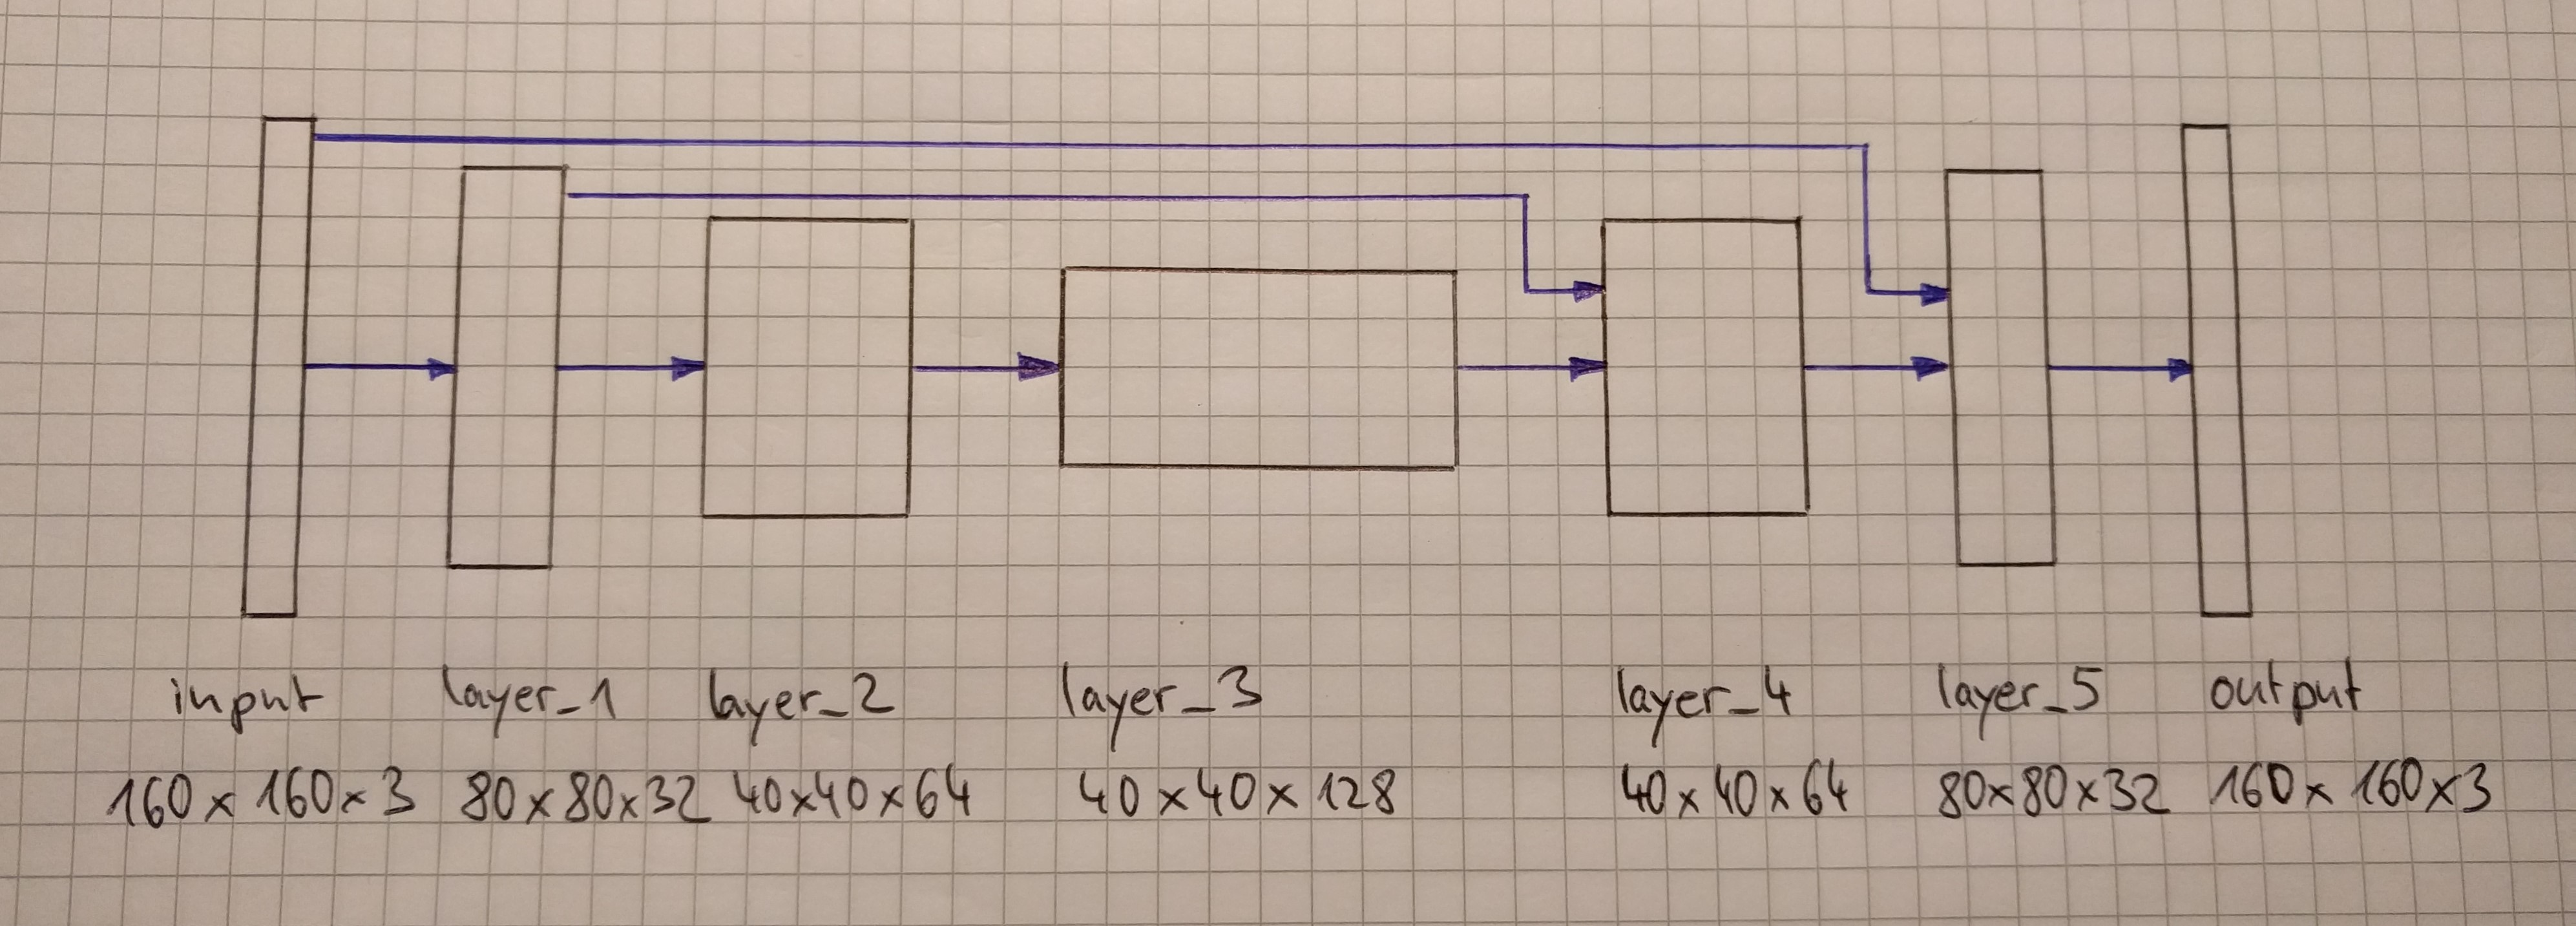
\includegraphics[width=\textwidth]{images/network_architecture.jpg}}
\caption[Diagram of FCN model]{Diagram of FCN model. Rectangles represent input/output layers and encoder/decoder blocks. Blue arrows represent connections. Layer names follow the notebook \href{https://github.com/S2H-Mobile/RoboND-DeepLearning-Project-Solution/blob/master/code/model_training.ipynb}{\texttt{model\_training.ipynb}}. For further model properties see table \ref{tbl:fcn_architecture}. The internal structure of the blocks is not shown in this diagram.}
\label{img:reference_architecture}
\end{figure}

{\renewcommand{\arraystretch}{2}%
\begin{table}
\centering
\begin{tabular}{|l|c|c|c|c|}
\hline 
Run & 1 & 2 & 3 & 4 \\
\hline
\multicolumn{5}{l}{Architecture}\\
\hline
Decoder convolutions & 2 & 1 & 2 & 1 \\
Maximum depth   & $128$ & $128$ & $256$ & $256$ \\
\hline
\multicolumn{5}{l}{Evaluation: Final Score}\\
\hline
Run \texttt{a} & 0.3908 & 0.3213 & 0.3834 & 0.3338 \\
Run \texttt{b} & 0.4277 & 0.3576 & 0.3955 & 0.4030 \\
\hline
%Average & 0.4093 & 0.3395 & 0.3894 & 0.3684 \\
Average $\pm$ deviation & $0.41 \pm 0.02$ & $0.34 \pm 0.02$ & $0.39 \pm 0.01$ & $0.37 \pm 0.04$ \\
\hline 
\end{tabular}
\caption[Architecture experiment]{Results of the architecture experiment. Maximum depth refers to the filter size of the $1 \times 1$ convolution layer. Learning rate is $0.005$. Batch size is $32$. Network configurations are trained over $10$ epochs with $200$ steps. The final scores are rounded to four significant digits for the individual runs and two significant digits for the average and deviation over the runs.}
\label{tbl:architecture_experiments}
\end{table}

\subsection{Hyperparameter Tuning}
I tested the reference architecture described in section \ref{sec:reference_architecture} with a variety of values for the learning rate, the batch size and number of epochs. I used the reference data sets for training, validation and evaluation. The results of this experiment are given in table \ref{tbl:hyperparameter_tuning}. The corresponding model files can be found in the \texttt{weights} directory named as \texttt{model\_weights\_tune\_n} where \texttt{n} is the number of the run.

{\renewcommand{\arraystretch}{2}%
\begin{table}
\centering
\begin{tabular}{|l|c|c|c|c|c|c|}
\hline 
Run & 1 & 2 & 3 & 4 & 5 & 6 \\
\hline  
\multicolumn{7}{l}{Hyperparameter Values}\\
\hline
learning rate    & 0.008 & 0.008 & 0.008 & 0.008 & 0.005 & 0.005 \\
batch size       & 20    & 32    & 32    & 32    & 32    & 32    \\
number of epochs & 4     & 4     & 10    & 16    & 16    & 50    \\
steps per epoch  & 200   & 200   & 200   & 200   & 200   & 200   \\
\hline 
\multicolumn{7}{l}{Evaluation}\\
\hline
final score & 0.3198 & 0.4009 & 0.4260 & 0.4054 & 0.4387 & 0.4285 \\
\hline 
\end{tabular} 
\caption[Hyperparameter tuning experiment]{Results of the hyperparameter tuning experiment on the reference architecture (see figure \ref{img:reference_architecture}) using the reference data sets for training, validation and evaluation.}
\label{tbl:hyperparameter_tuning}
\end{table}

I started with default values from the lab and trained $4$ epochs. In the subsequent runs I increased the number of epochs and observed an improving final score. At $16$ epochs I noticed the final score dropping. So I decreased the learning rate in order to prevent overfitting. I ran experiment 5 with a learning rate of $0.005$ and the final score improved.

In run $6$ I increased the number of epochs further to $50$. The training curve of this run is shown in figure \ref{img:training_curves_tune_6}. The final score did not improve compared to the previous run.

From the results of the tuning experiment I deduced that the current best learning rate to work with is $0.005$. 

I left the number of steps per epoch at $200$, in future work this can also be tuned. The number of epochs can be increased and the number of steps decreased.

\begin{figure}
\noindent
\makebox[\textwidth]{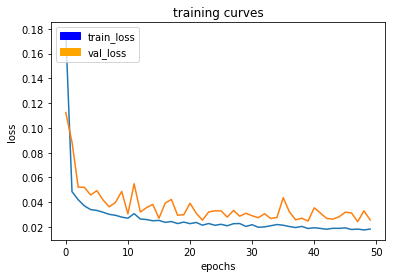
\includegraphics[width=\textwidth]{images/training_curve_tune_6.png}}
\caption[Training curves for tuning run 6]{Training curves for tuning run $6$ with $50$ epochs at a learning rate of $0.005$.}
\label{img:training_curves_tune_6}
\end{figure}

\subsection{Training with additional data}
\label{sec:training_additional_data}
When I had explored several configurations of architecture and hyperparameter values, I started to use the data collected in the simulator. I took the reference network as shown in figure \ref{img:reference_architecture} and the hyperparameter values of tuning run $6$ (see table \ref{tbl:hyperparameter_tuning}). I trained this configuration on the combined data (see section \ref{sec:data_collection} for the data collection process). The results are given in table \ref{tbl:collected_data_experiment}.

{\renewcommand{\arraystretch}{2}%
\begin{table}
\centering
\begin{tabular}{|l|c|c|}
\hline 
Run & 1 & 2 \\
\hline  
\multicolumn{3}{l}{Hyperparameter Values}\\
\hline
learning rate    & 0.005 & 0.005 \\
batch size       & 32    & 32    \\
number of epochs & 16    & 50    \\
steps per epoch  & 200   & 200   \\
\hline 
\multicolumn{3}{l}{Evaluation}\\
\hline
final score & 0.3734 & 0.4044  \\
\hline 
\end{tabular}
\caption[Collected data experiment]{Results of the collected data experiment using the collected data set for training and the reference data sets for validation and evaluation. The experiment is performed on the network configuration described in \ref{tbl:fcn_architecture} and figure \ref{img:reference_architecture}.}
\label{tbl:collected_data_experiment}
\end{table}

\section{Results}
The model trained in tuning run $6$ (last column in table \ref{tbl:hyperparameter_tuning}) shows the best performance. It reaches final scores of approximately $0.43$. Therefore I submit the corresponding weight file \texttt{model\_weights\_tune\_6}.

Against expectations, gathering additional data did not have a significant effect on the network performance. I assume that this can be improved by collecting much more image sequences, where the hero is present in the camera image, and with more variation in the background scenery.

\subsection{Future Enhancements}
The following improvements of the network architecture, the hyperparameter tuning and the data collection process seem to be promising next steps to increase the performance of the model.
\begin{itemize}
\item Tune the number of steps per epoch. Increasing the number of epochs and decreasing the number of steps per epoch might increase the model performance while taking the same training time.
\item Experiment with learning rate decay and early stopping. Take full advantage of all the options provided by the \href{https://keras.io/optimizers/}{Keras optimizers package}.
\item Use \texttt{sklearn.grid\_search.GridSearchCV} to automate the hyperparameter tuning experiments.
\item Collect more image data, possibly with the target being present in a higher fraction of the camera images.
\item In the decoder block, use transpose convolutions (see \href{https://keras.io/layers/convolutional/#conv2dtranspose}{Keras}) instead of the less accurate bilinear upsampling technique.
\end{itemize}

Regarding the task of detecting more types of objects (dog, cat, car, etc.) I did some research and found the \href{https://github.com/matterport/Mask_RCNN}{Mask R-CNN} project. As a first step I let that model run object detection on the image \texttt{5\_run6cam1\_00197.jpeg} from the validation data set. The result is encouraging, since besides the hero person a potted plant is detected as well, see figure \ref{img:example_mask_rcnn}.

I'm curious to compare both projects, their architecture and data sets, for example train the Follow Me!\ network on the multiple-object images provided there and vice versa.

\begin{figure}
\noindent
\makebox[\textwidth]{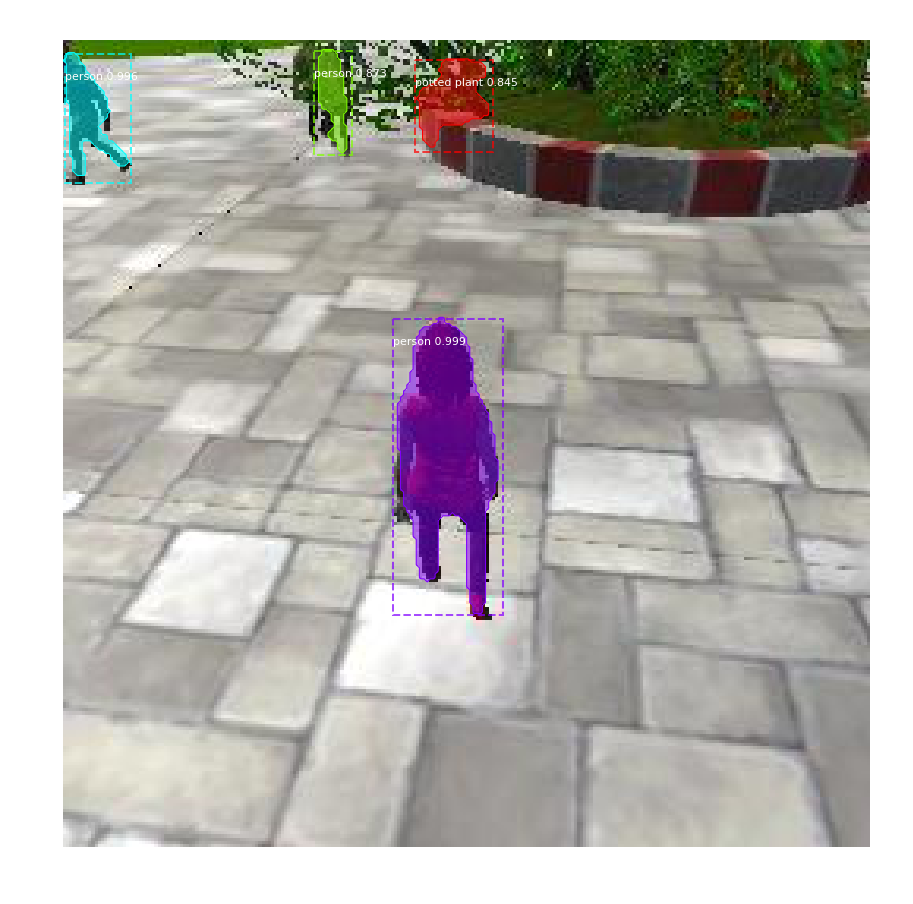
\includegraphics[width=\textwidth]{images/example_mask_rcnn.png}}
\caption[Demo run for detecting object types]{Result of demo run for recognizing multiple objects using the Mask R-CNN model.}
\label{img:example_mask_rcnn}
\end{figure}

\begin{thebibliography}{3}
\bibitem{CS231n}
 \href{http://cs231n.stanford.edu/}{Stanford CS231n}
 \textit{Convolutional Neural Networks for Visual Recognition},
 \href{http://cs231n.github.io/convolutional-networks/}{Class Notes on Convolutional Neural Networks}

\bibitem{Xception}
  Fran{\c{c}}ois Chollet,
  \textit{Xception: Deep Learning with Depthwise Separable Convolutions},
  CoRR, abs/1610.02357,
  2016,
  \href{http://arxiv.org/abs/1610.02357}{http://arxiv.org/abs/1610.02357}

\bibitem{MobileNets}
  Andrew G. Howard and
               Menglong Zhu and
               Bo Chen and
               Dmitry Kalenichenko and
               Weijun Wang and
               Tobias Weyand and
               Marco Andreetto and
               Hartwig Adam,
  \textit{MobileNets: Efficient Convolutional Neural Networks for Mobile Vision Applications},
  CoRR, abs/1704.04861,
  2017,
  \href{http://arxiv.org/abs/1704.04861}{http://arxiv.org/abs/1704.04861}
\end{thebibliography}

\end{document}